
\begin{frame}[fragile]
  \frametitle{\shortt:  Experimento 1}
    \begin{block}{Problemas de comunicación}
        Los niños suelen tener dificultades articulando hipótesis causales explícitamente, por lo que se diseño un experimento que sólo requiere criterios positivos/negativos.
    \end{block}
    \begin{center}
    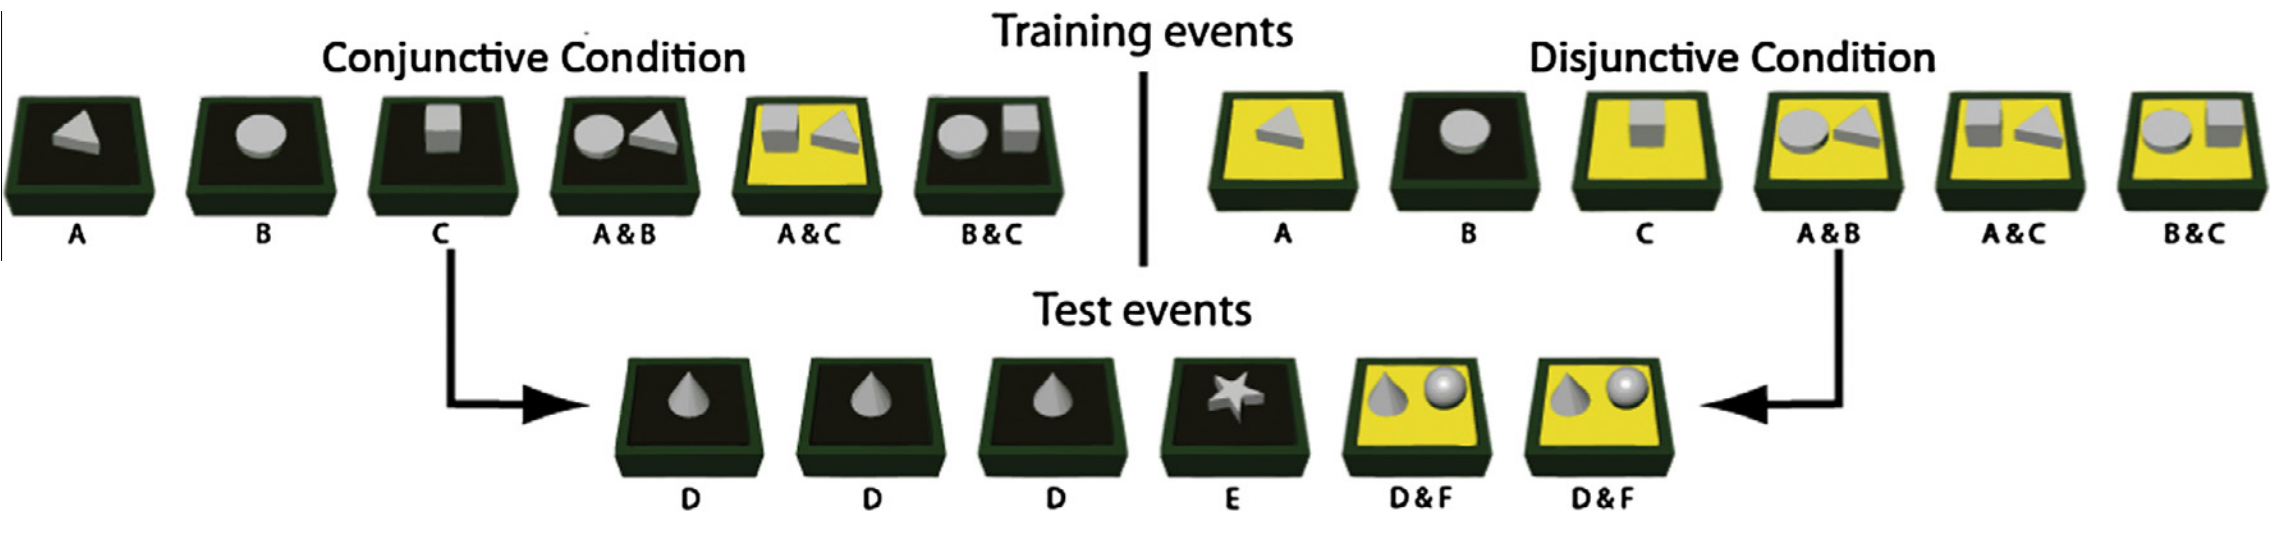
\includegraphics[scale=0.25]{images/experiment1.png}
    \end{center}
\end{frame}

\begin{frame}[fragile]
  \frametitle{\shortt: Experimento 1}
    \begin{block}{Objetivos del Experimento}
    \begin{itemize}
    \item El entrenamiento no genera efecto en niños: Lleva a pensar en que la habilidad de formar relaciones causales es una consecuencia en el aprendizaje a fines de la niñez.
    \item Los niños y adultos están predispuestos a relaciones disyuntivas:  Esta predisposición es de desarrollo temprano en el aprendizaje.
    \item Los niños pueden aprender ambas fórmas indistintamente: Por lo tanto la predisposición disyuntiva se debe al aprendizaje y experiencia de los adultos.
    \end{itemize}
    \end{block}
\end{frame}

\begin{frame}[fragile]
  \frametitle{\shortt: Experimento 1}
    \begin{block}{Resultados}
    \begin{center}
    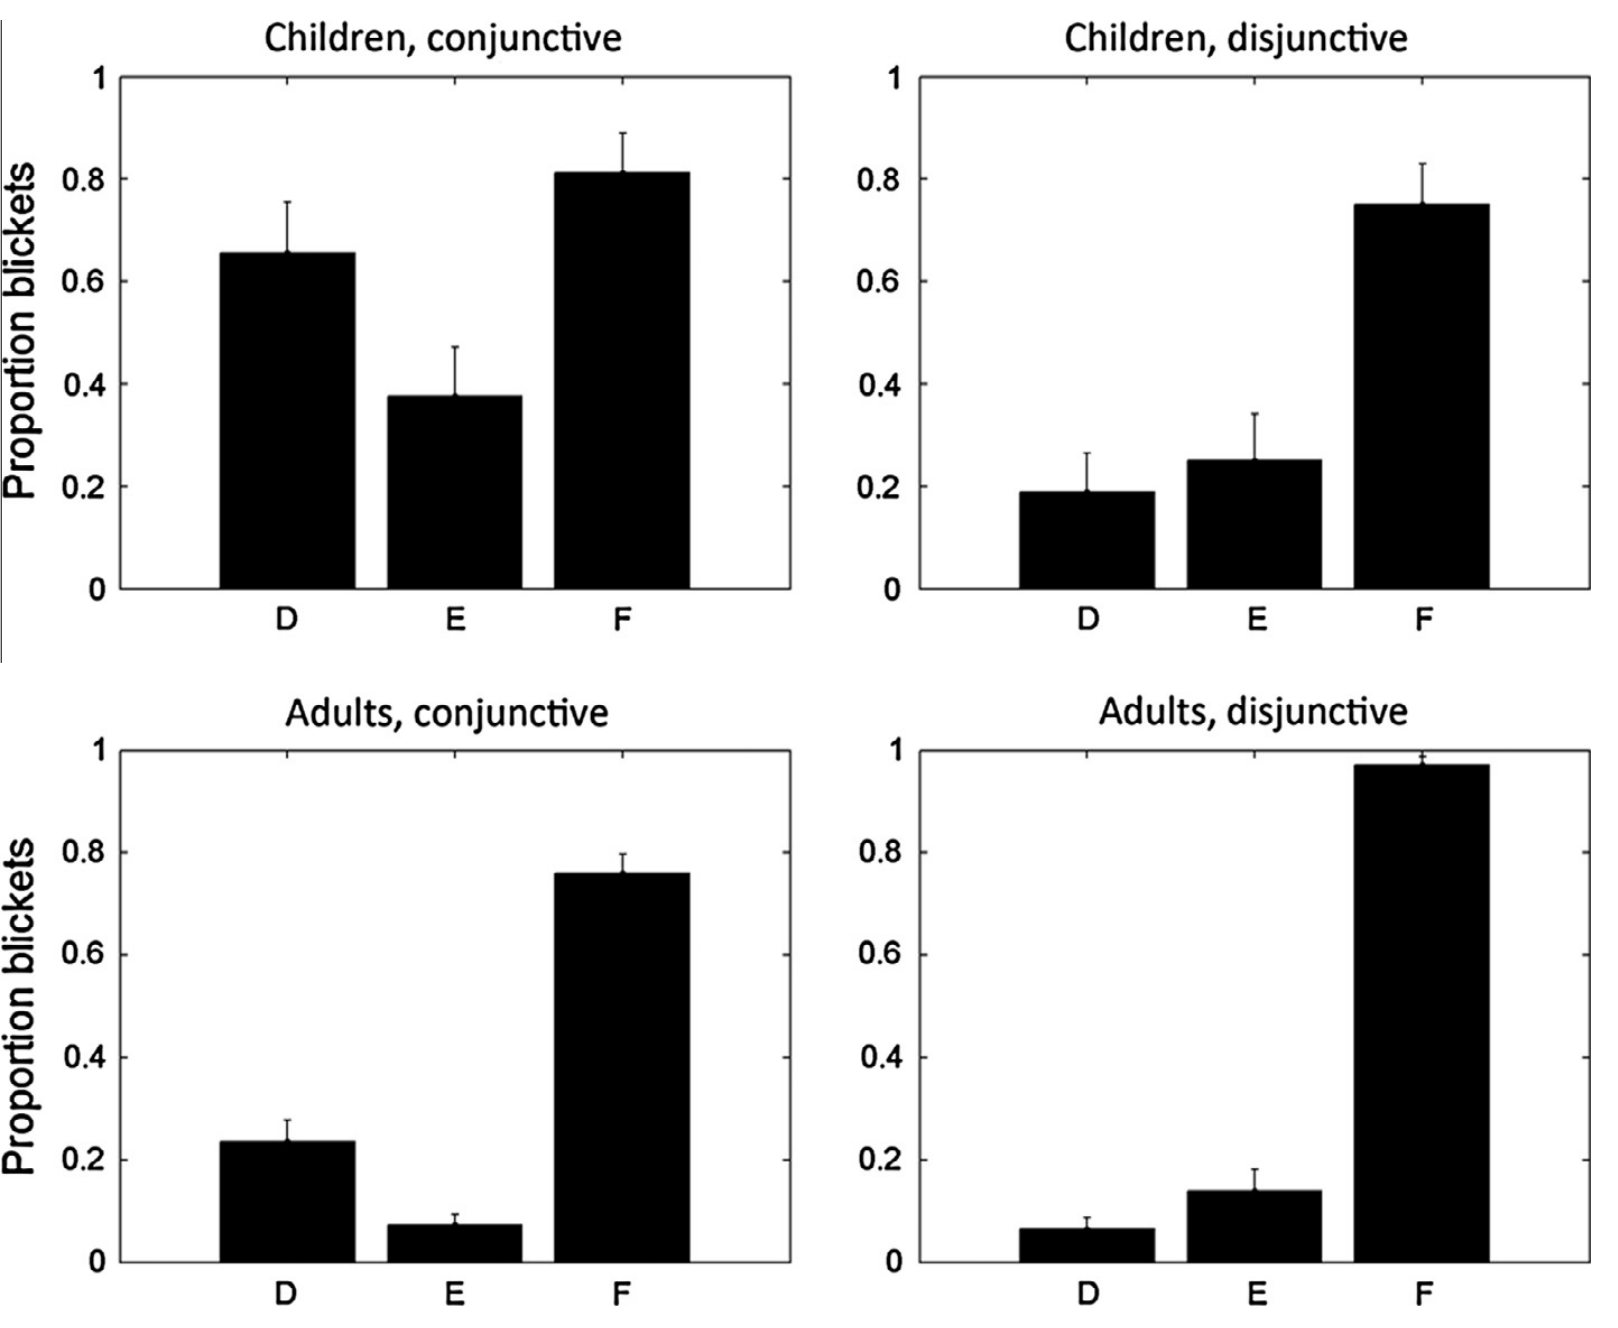
\includegraphics[scale=0.25]{images/experiment1results.png}
    \end{center}
    \end{block}
\end{frame}

\begin{frame}[fragile]
  \frametitle{\shortt: Experimento 1}

    \begin{block}{Resultados}

        \begin{itemize}
        \item Los niños utilizaron los datos de entrenamiento en ambas condiciones.
        \item Niños y adultos se comportaron de la misma forma con la forma disyuntiva.
        \item Los niños aseguran que D y E podrían ser un blicket en la forma conjuntiva.
        \item Los adultos no tomaron en cuenta el entrenamiento conjuntivo y sólo aceptaron a F como respuesta.
        \end{itemize}
        
        Esto afirma las hipótesis sobre el experimento.
    \end{block}

\end{frame}

\begin{frame}[fragile]
  \frametitle{\shortt: Experimento 1}

    \begin{block}{Interpretación}
    \begin{itemize}
    \item Los niños pueden ser más propensos a indicar que cualquier objeto es un blicket.
    \item Los niños se confundieron con el entrenamiento conjuntivo y respondieron sobre D y E, respondiendo randómicamente.
    \item Falta de información sobre E pudo implicar que no sea elegido como blicket.
    \item No se testean los conocimientos causales si no el uso de términos como "blicket", por lo que se utiliza la idea de "blicketness" para incentivar se considere la posibilidad conjuntiva.
    \end{itemize}
    \end{block}
    \begin{block}{Problemas}
    Si la última explicación es correcta, niños y adultos deberían comportarse de igual forma cuando se les pide activar la máquina.
    Sin embargo si infieren diferentes formas causales en las dos condiciones, deberían usar sólo un bloque para activarla en la forma disyuntiva, pero deberían intentar con combinaciones en la forma conjuntiva.
    De igual forma los adultos usarían sólo un bloque para activar la máquina en ambas condiciones.
    
    Para eliminar hipótesis alternativas, se realizó un segundo experimento.
    \end{block}



\end{frame}

\begin{frame}[fragile]
  \frametitle{\shortt: Metodología}

Experimento 2, diferencias:

\begin{itemize}
\item Se pregunta que objetos usarían para activar la máquina.
\item Se modificaron los eventos de prueba para que todos los objetos tengan la misma probabilidad de activar la máquina. (D - D - D - E - DF+ - DEF+ - DF+ ).
\item Se agrega un nuevo objeto G, al que se lo llama \textit{novel object} que no participa en el experimento.
\item Se agrega un nuevo baseline en donde se omite el entrenamiento de los individuos.
\item Se simplifica el procedimiento dando sólo una prueba en vez de dos, pero se repite el entrenamiento dos veces.
\end{itemize}


\end{frame}

\begin{frame}[fragile]
  \frametitle{\shortt: Metodología}

Experimento 2, predicciones:

\begin{itemize}
\item Los niños en el caso disyuntivo deberían devir que F es blicket y los demás no. Indicar que con un solo objeto se activa la máquina.
\item Los niños en el caso conjuntivo deben decir que F y D son blickets y dudar sobre E. Para activar la máquina precisan un conjunto de objetos.
\item 
\end{itemize}


\end{frame}